 % -*- encoding: UTF8 -*-
%
%%*****************************************************************************
%%				Fabrication and Assembly										                                        
%%*****************************************************************************
\chapter{Implementation}
\label{Ch:Fab}	

This chapter details the implementation of the probe shown in \autoref{fig:overview}, which serves as a demonstrator of the fiber scanner design and evaluation tool of the optical performance of the OCT beam path.

\begin{figure}[h!]\centering 
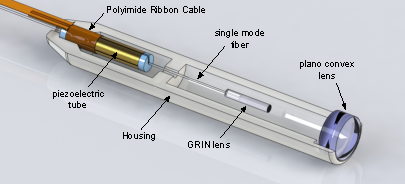
\includegraphics[width=\columnwidth]{figures/40_Fabrication/overview.pdf}
      \caption{CAD of the single modality demonstrator with the top of the housing removed. Total length: \SI{9}{\milli\meter}.}
      \label{fig:overview}
\end{figure}

The design can be summarized as follows: The piezoelectric actuator has four outer gold electrodes to control the lateral movement of the scanner. The addressing of these electrodes is realized by a ribbon cable, which is wrapped around the piezoelectric tube. The single mode fiber is centered in the piezoelectric tube and the GRIN lens bonded to the tip of this fiber. This arrangement enables a compact fiber scanner with a total length of \SI{9}{\milli\meter} and a resonance frequency of \SI{750}{\hertz} optimized for an OCT system with an A-Scan repetition rate of \SI{100}{\kilo\hertz}.

The following paragraphs describe the manufacturing process and assembly of the most relevant components of the probe, beginning with the fabrication of the polyimide electrodes used for contacting the piezoelectric tube and proceeding with details of the necessary assembly steps to fabricate the scanner, leading to the assembly of the complete probe.


%%*****************************************************************************
\section{Polyimide Electrodes}
%%*****************************************************************************
The first challenge that appears in the manufacturing of the scanner lies in contacting the four external electrodes of the piezoelectric tube. 

Due to the small diameter of the tube (\SI{800}{\micro\meter}), creating a reliable interface between the driving circuit and its electrodes is not trivial. Other piezoscanner implementations use soft soldering and insulated copper wires \cite{Lee2010}, \cite{Meinert}, \cite{Huo2010}, but the soldering process can damage the piezoelectric material, as it is exposed to temperatures above its Curie temperature. This method also increases the diameter of the actuator significantly, as a solder blob is needed. %Furthermore, it requires welding by hand in a \SI{600}{\micro\meter} curved electrode.

Instead, this design uses a polyimide ribbon cable which is wrapped around the piezotube and addresses its four external electrodes using vias. Its geometry, cross section and application over the tube is depicted in Figure \ref{fig:piRolled}, while \autoref{fig:piRender} shows its complete design.

\begin{figure}[h!]\centering 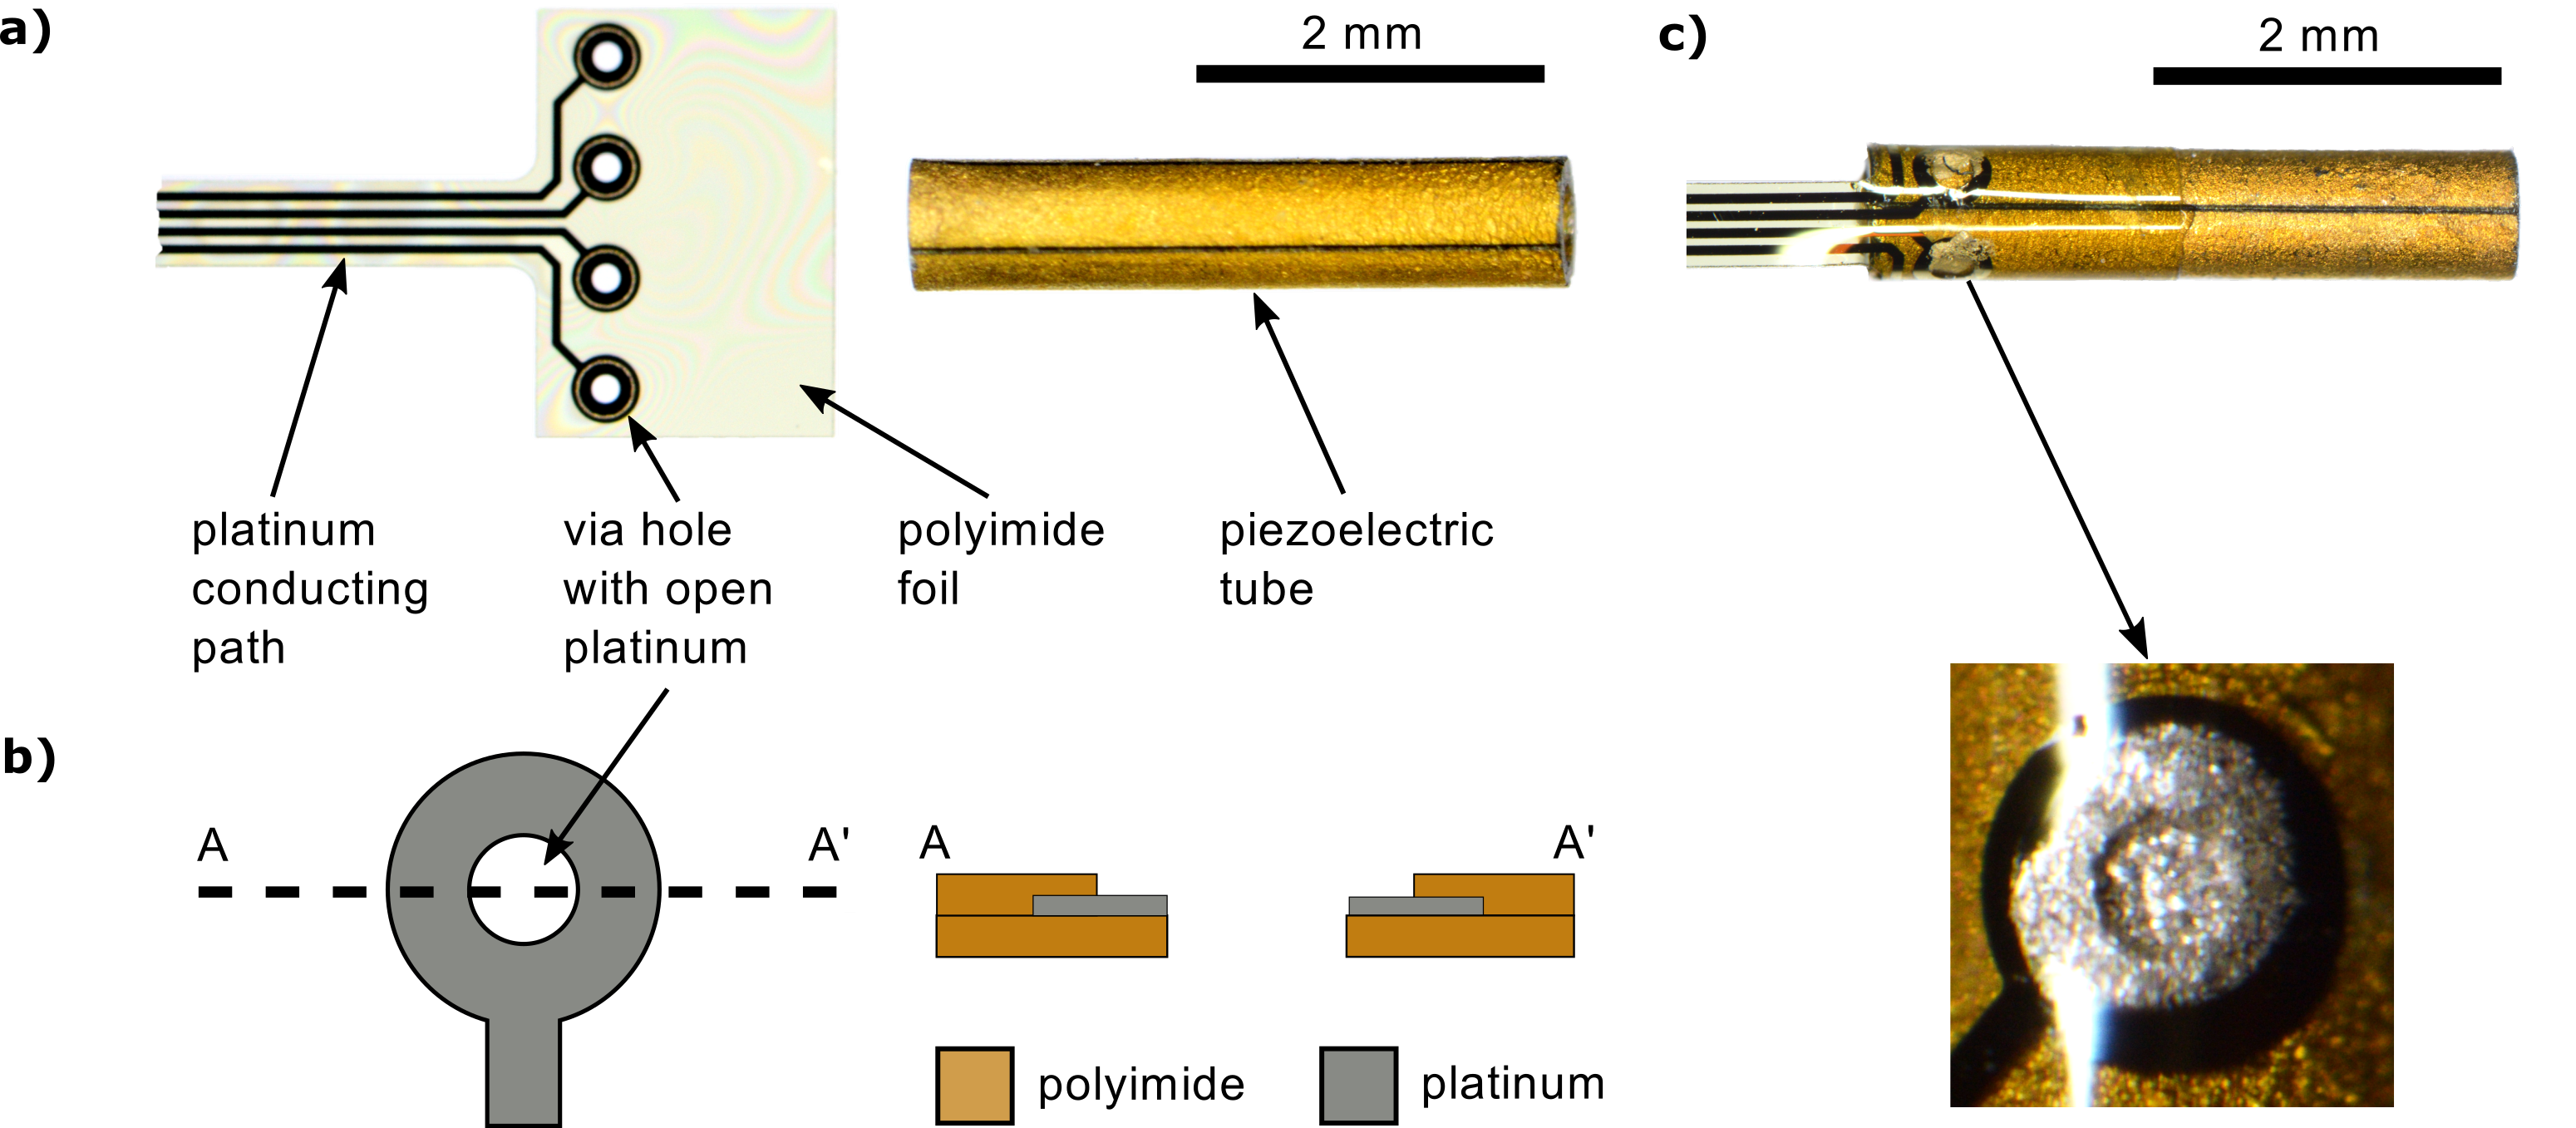
\includegraphics[width=15cm]{figures/40_Fabrication/PI/tubeFoilH.png}
      \caption{Polyimide electrode design.
      \textbf{a)} \textit{Left}: Photo of the polyimide ribbon cable with four vias to contact the four gold electrodes of the piezoelectric tube. \textit{Right}: Piezoelectric tube.
      \textbf{b)} Schematic of one via and its cross section. The platinum around the via is partly uncovered to improve the electrical connection between the cable and the piezoelctric tube.
      \textbf{c)} Photography of a polyimide ribbon cable, wrapped around the piezoelectric tube that is electrical connected through the vias by conductive glue.
      \textbf{d)} Microphotograph of the via after bonding with conductive glue.}
      \label{fig:piRolled}
\end{figure}

It is manufactured using a cleanroom process similar to the one used for cuff electrodes for nerve stimulation \cite{Rodriguez2000} and consists of platinum tracks and via holes embedded in a polyimide substrate. One end the cable is shaped to fit a zero insertion force (ZIF) connector. The other end can be rolled around the piezoelectric tube, allowing the bonding to its gold electrodes using conductive glue (Araldite 2020 with 80\% wt. silver particles).

\begin{figure}[h!]\centering 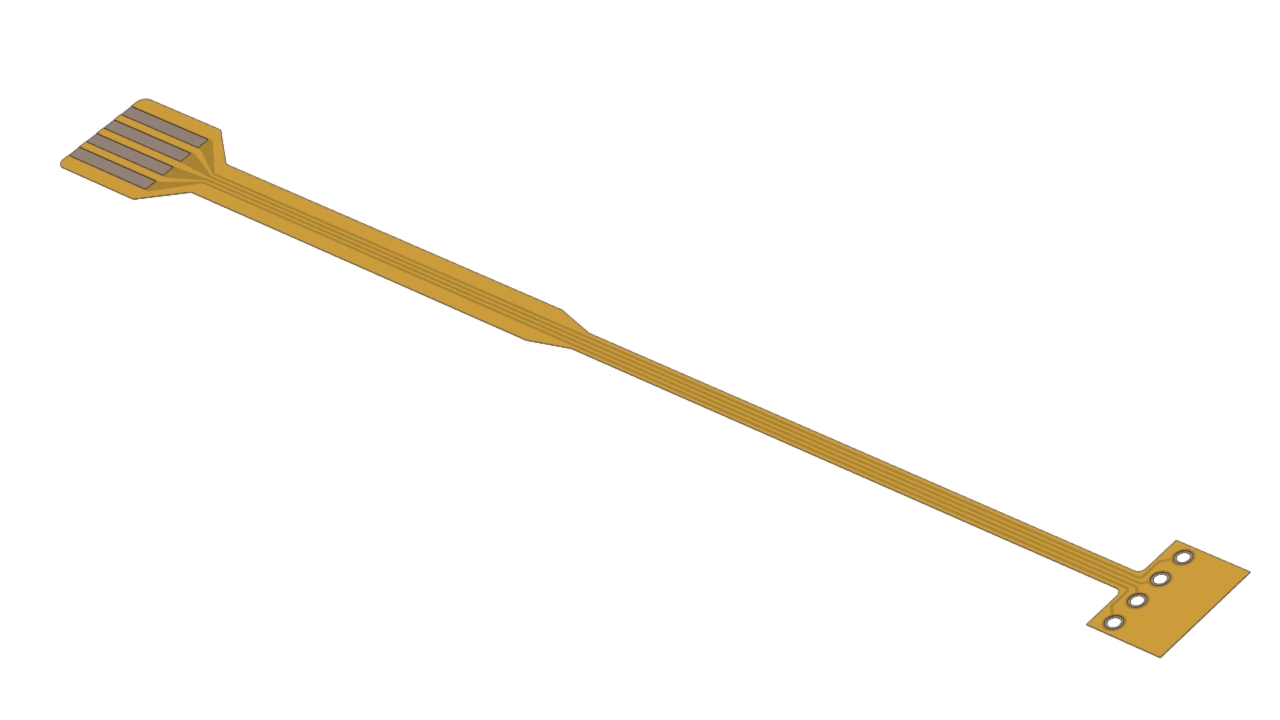
\includegraphics[width=15cm]{figures/40_Fabrication/PI/render.JPG}
      \caption{Render of a manufactured polyimide electrode. The left side fits a ZIF connector, the right side is rolled around the piezoelectric tube to address its electrodes.}
      \label{fig:piRender}
\end{figure}



\subsection{Cleanroom processing}
The polyimide ribbon cables are manufactured and singulated at wafer level. The process involves spin coating a \SI{5}{\micro\meter} layer of polyimide, over which \SI{100}{\nano\meter} of platinum is sputtered and then patterned by liftoff, defining the conductive traces. On top of it, a second \SI{5}{\micro\meter} layer is spincoated. Finally, the vias, openings and external shape are patterned through reactive ion etching (RIE). This process is described in Figure \ref{fig:piProcess} and the resultant wafer in \autoref{fig:piwafer}.


\begin{figure}[h!]\centering 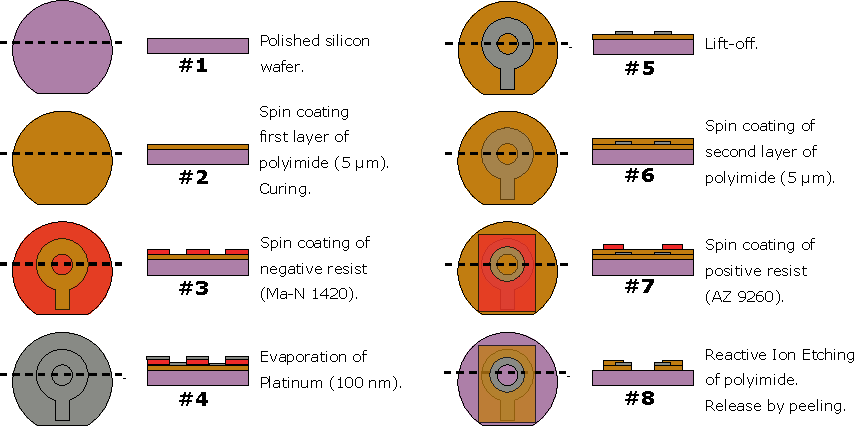
\includegraphics[width=15cm]{figures/40_Fabrication/PI/processH.pdf}
      \caption{Illustration of the fabrication of a polyimide-platinum via. The first column shows the top view of the wafer, while the cross section is depicted in the second column.}
      \label{fig:piProcess}
\end{figure}

\begin{figure}[h!]\centering 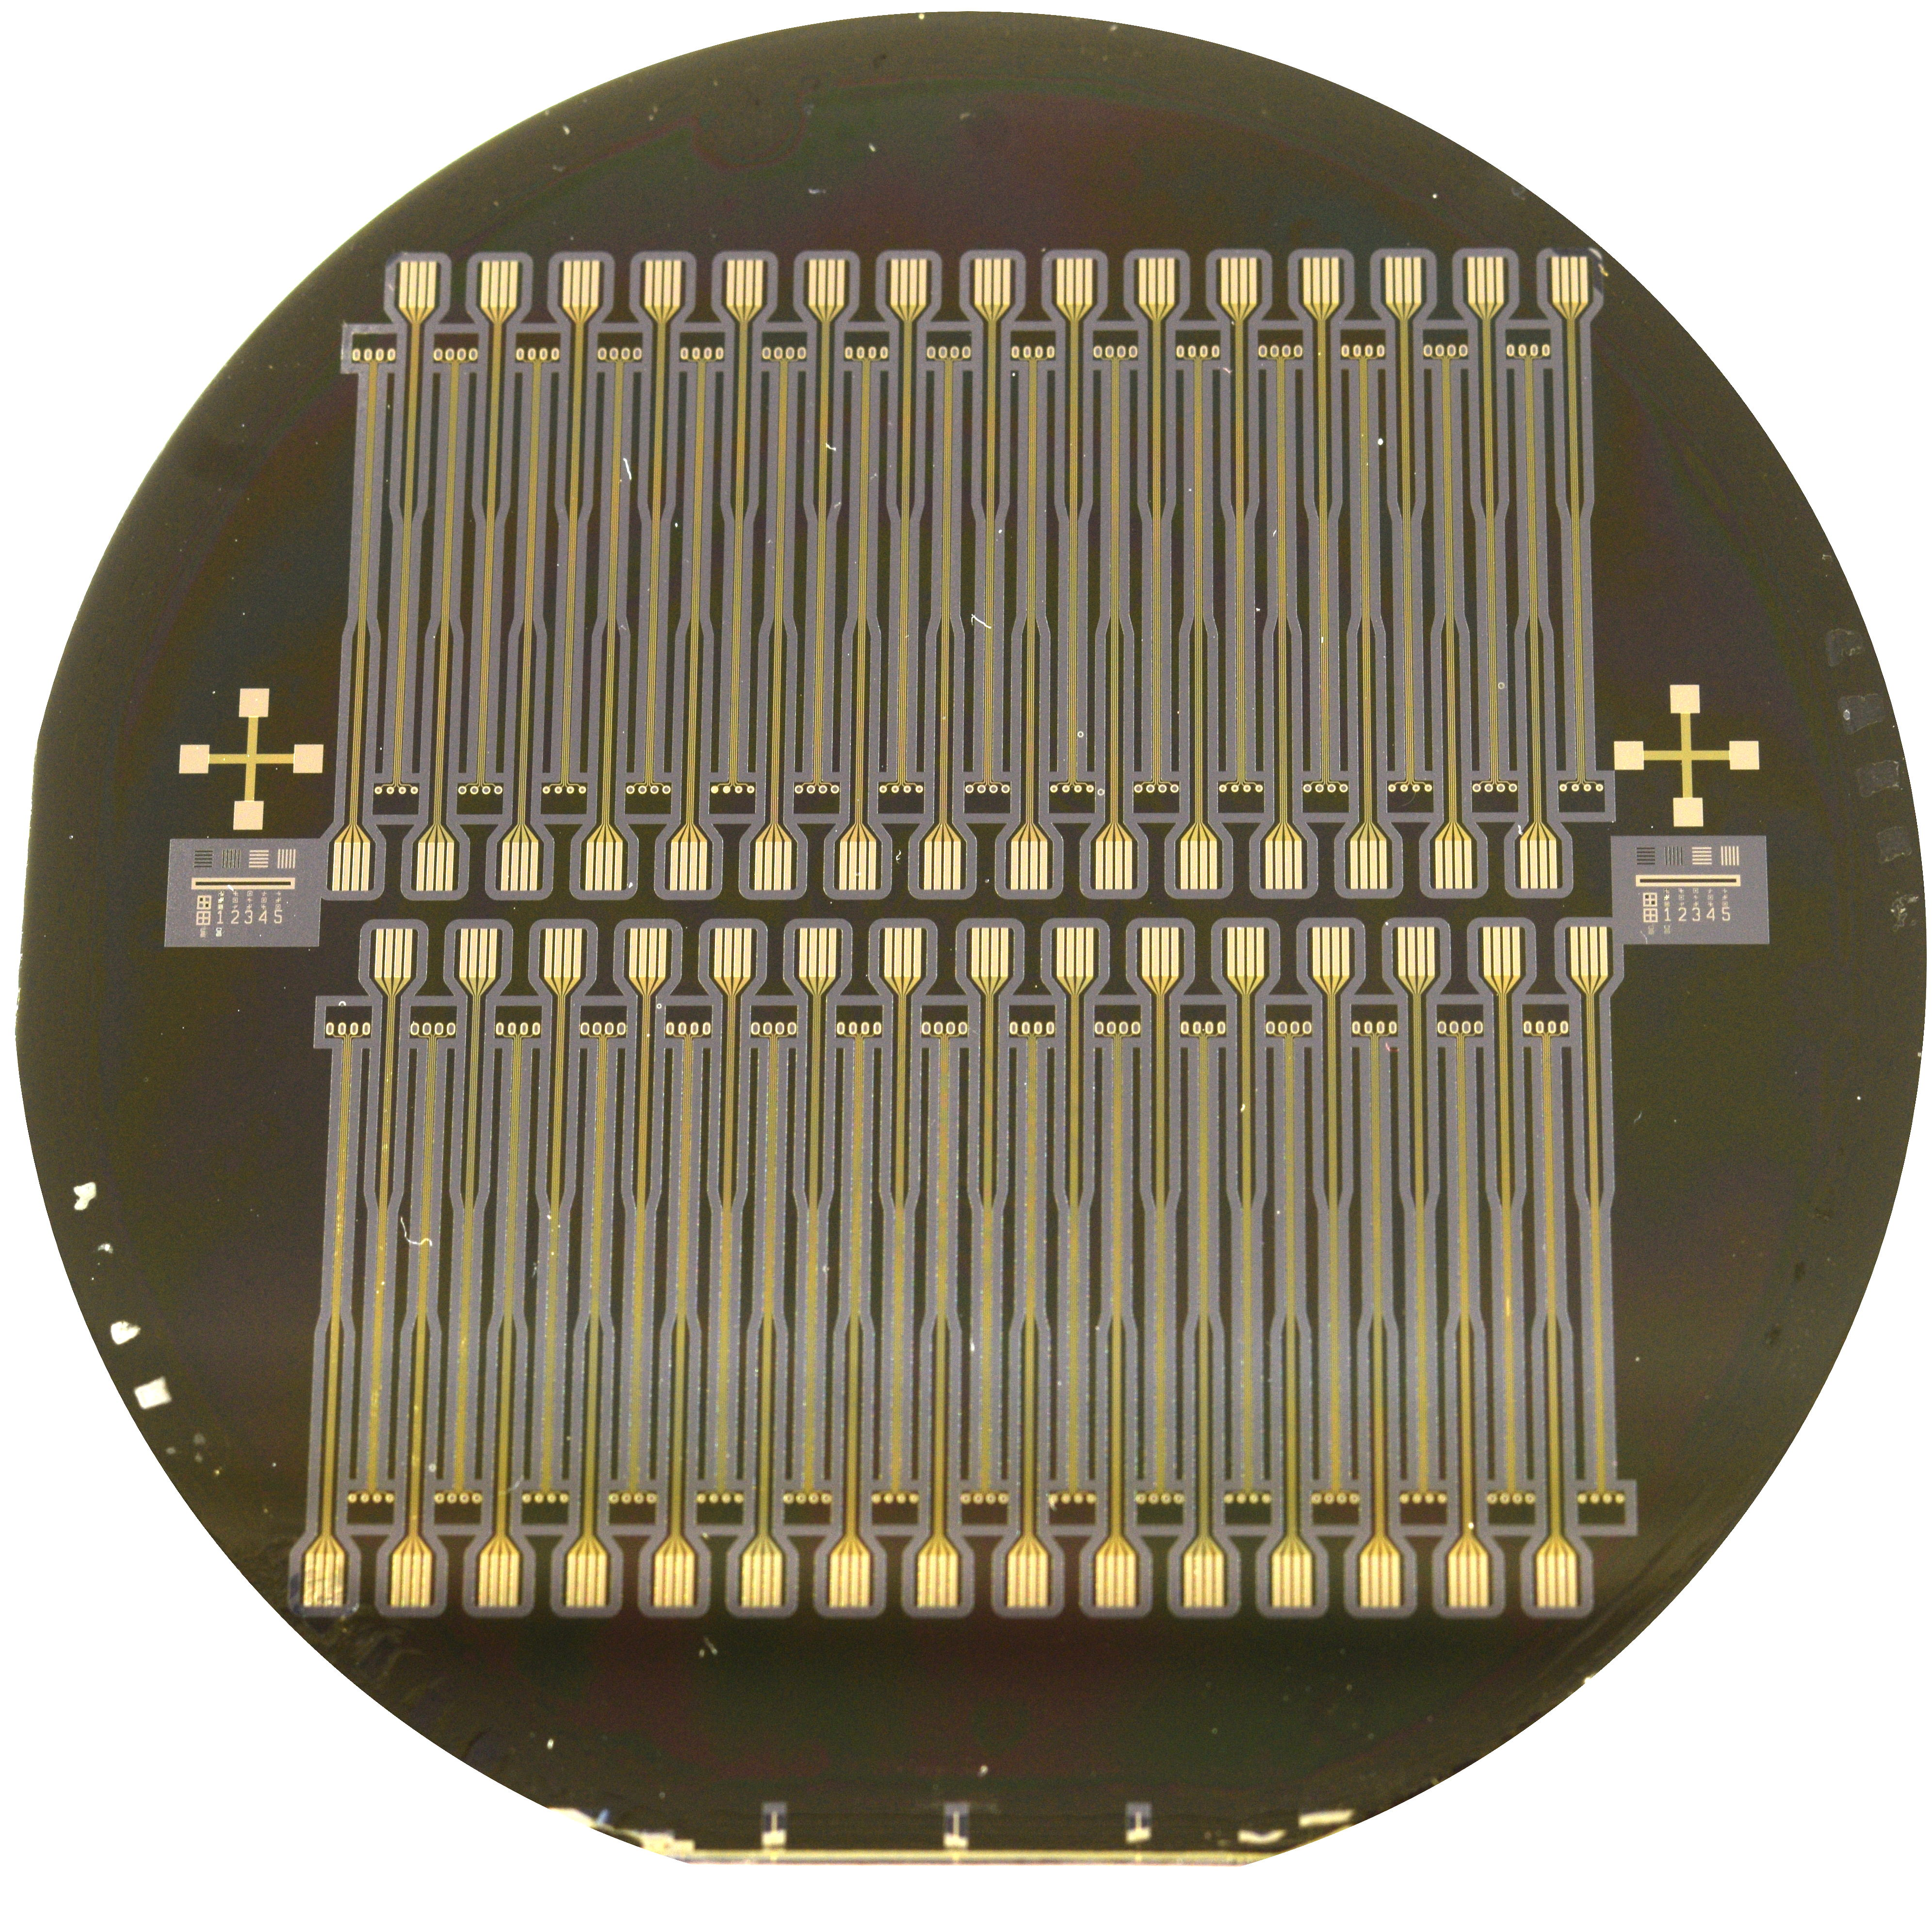
\includegraphics[width=10cm]{figures/40_Fabrication/PI/wafer.JPG}
      \caption{True scale photography of a \SI{100}{\milli\meter} wafer containing 60 polyimide electrodes.}
      \label{fig:piwafer}
\end{figure}

%%*****************************************************************************
\clearpage
\section{Fiber-GRIN Bonding}
\label{sec:fiberGRIN}
%%*****************************************************************************
Another step that has to be performed before the final assembly of the probe is to bond the GRIN lens to the end of the fiber optically and mechanically. This interface is critical: first, because it is subjected to very high forces due to the oscillation of the scanner, and second, because any angular or displacement error would degrade the optical quality.

To overcome these challenges, fiber and GRIN lens are aligned together using a custom made, KOH-etched silicon alignment tool. The geometry of the KOH-etched grooves together with the cylindrical shape of both components allow the precise angle and position control of the fiber and GRIN lens. Once in place, a drop of index-matched UV-curable glue (NOA 76) bonds the components together. The wetting behavior and surface tension of the glue create a symmetrical wedge which provides extra mechanical integrity, as can be seen in \autoref{fig:fiberGRINglue}.

\begin{figure}[h!]\centering \includegraphics{figures/40_Fabrication/FiberGRIN/fiberGRINglue.pdf}
      \caption{\textbf{a)} Photography of the tip of the fiber (right) and GRIN lens (left) seating in the alignment tool.
      \textbf{b)} Bonding with UV-curable adhesive.}
      \label{fig:fiberGRINglue}
\end{figure}

%\begin{figure}[h!]\centering 
\includegraphics[width=10cm,draft]{figures/foo.png}
%      \caption{Cross section with dimensions}
%      %\label{}
%\end{figure}



%%*****************************************************************************
\section{3D Printed Housing}
%%*****************************************************************************

The bimodal probe is designed to be assembled using the silicon bench technology \cite{Kretschmer}. But for the demonstrator, a process with reduced complexity, which allows faster design adjustments has been tested: using a 3D printed polymer structure for both assembly and housing.

This is possible because, even though the dimensional accuracy of the printed housing is lower than its silicon counterpart, the optical components of the demonstrator allow relatively high placement tolerances, as the beam is collimated in the region between GRIN lens and objective lens. This way, simple alignment structures which are 3D-printed within the housing allow the proper placement of all components, as shown in \autoref{fig:housing}. The main dimensions of the housing are depicted in \autoref{fig:housingDim}.

\begin{figure}[h!]\centering \includegraphics[width=\columnwidth]{figures/40_Fabrication/Housing/housing.pdf}
      \caption{CAD (a) and photography (b) of the single modality probe with alignment features.}
      \label{fig:housing}
\end{figure}

\begin{figure}[h!]\centering 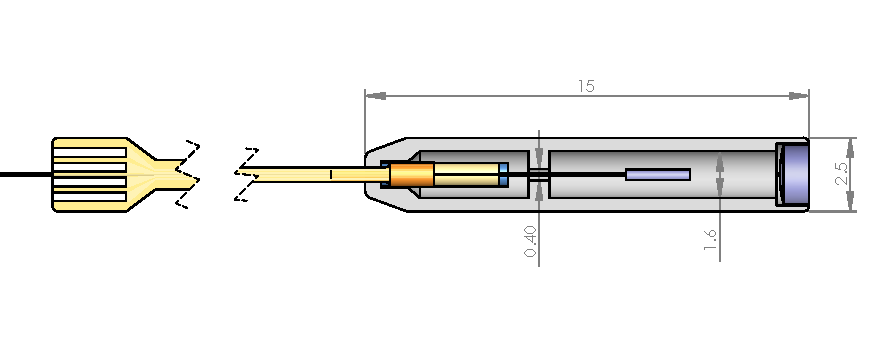
\includegraphics[width=\columnwidth]{figures/40_Fabrication/Housing/TopDrawing.pdf}
      \caption{Top view of the single modality probe showing the main dimensions of the housing.}
      \label{fig:housingDim}
\end{figure}

The housing is manufactured using a \textit{B9Creator} stereolithography printer, which allows the polimerization of an acrylic resin with a lateral resolution of \SI{30}{\micro\meter}.


%As an example, in order to center the piezotube in the housing, first the fiber is retracted so that the GRIN lens seats in the GRIN alignment structure (Figure \ref{fig:grinAlignment} left). This way the piezotube is aligned in the housing and, after being glued in place, it is possible to push the fiber so that the GRIN is at its proper distance (Figure \ref{fig:grinAlignment} right). 
%
%\begin{figure}[h!]\centering 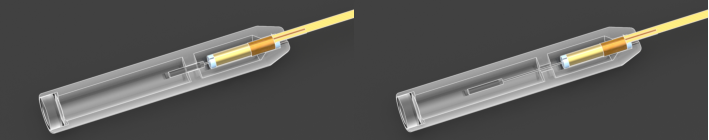
\includegraphics[width=\columnwidth]{figures/40_Fabrication/Housing/grinAlignment.pdf}
%      \caption{Alignment sequence of the piezotube-fiber-GRIN assembly in the housing. 
%      \textit{Left}: GRIN is retracted to allow the alignment.
%      \textit{Right}: Final position after gluing.}
%      \label{fig:grinAlignment}
%\end{figure}

%%*****************************************************************************
\section{Assembly}
%%*****************************************************************************

%\autoref{fig:exploded} shows the components upon which the demonstrator probe is built and the resultant assembly. 
%
%\begin{figure}[h!]\centering 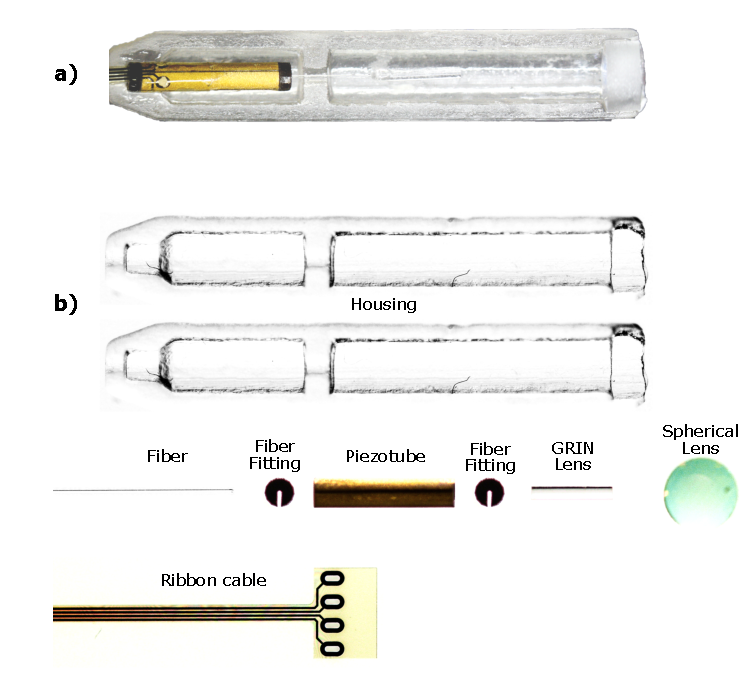
\includegraphics{figures/40_Fabrication/Assy/exploded.pdf}
%      \caption{\textbf{a)} Exploded view of the components which form the single modality probe.
%      \textbf{b)} Photograph of the assembled probe with the top half of the housing removed.}
%      \label{fig:exploded}
%\end{figure}


Once all the components are ready, the assembly is performed by hand using the multiple alignment features of the housing. The exploded view in \autoref{fig:exploded} shows the placement of the components prior to assembly, followed by the final encapsulation. This process is summarized as follows:

\begin{figure}[h!]\centering 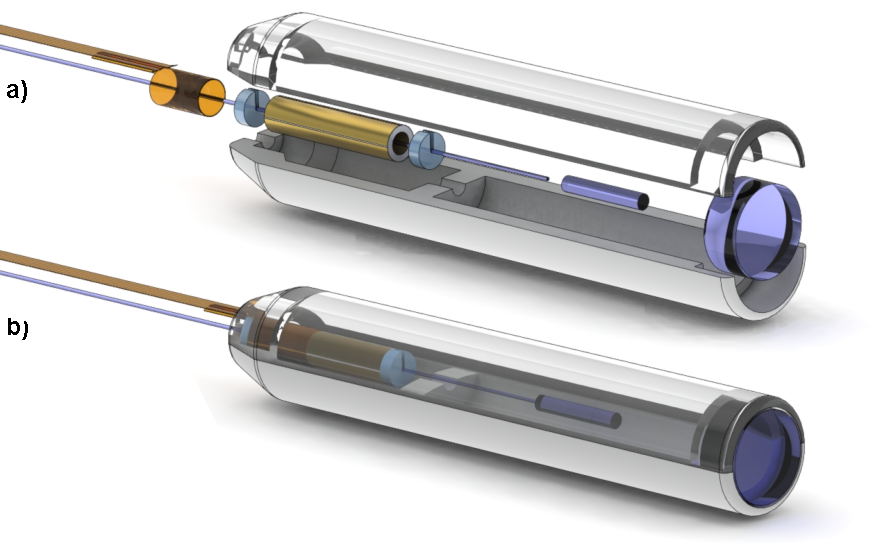
\includegraphics{figures/40_Fabrication/Assy/explodedRender/explodedRender.pdf}
      \caption{\textbf{a)} Exploded view of the components which form the single modality probe.
      \textbf{b)} Render of the complete probe after assembly.}
      \label{fig:exploded}
\end{figure}

\begin{enumerate}
\item The GRIN lens is bonded to the end of the fiber using the alignment tool (\autoref{sec:fiberGRIN}).
\item The GRIN-fiber assembly is slid through the piezotube and centered with FR-2 fittings, which are glued to the piezotube using cyanocrilate.
\item The piezotube-fiber-GRIN assembly is placed in the housing and glued in place using cyanocrilate with help of the alignment structures.
\item The planoconvex lens is placed in the bottom half of the housing and glued using UV-curable optical glue.
\item The probe is closed with the top half of the housing and sealed with UV-curable glue.
\end{enumerate}

